
\begin{figure}
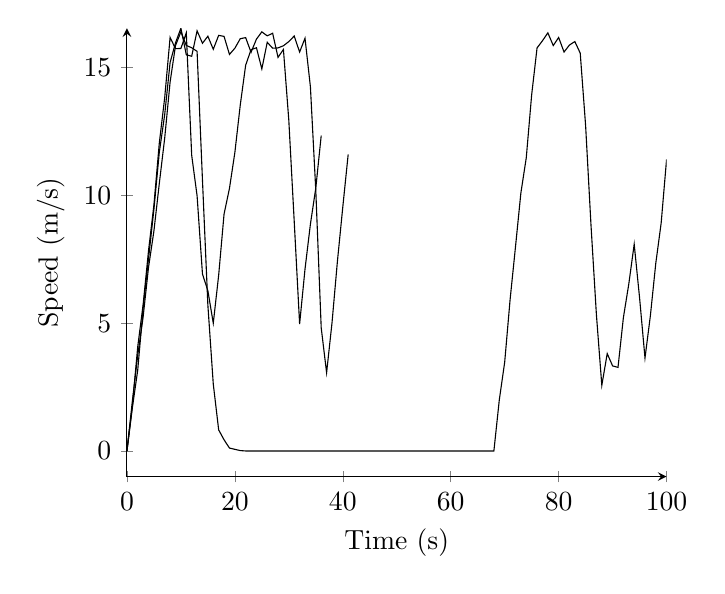
\begin{tikzpicture}
\begin{axis}[
legend style={anchor=west},
axis x line=bottom,
axis y line=left,
ymin=-1,
xlabel=Time (s),
ylabel=Speed (m/s),
]
\addplot[] coordinates {
(0, 0.0)
(1, 1.74415127432)
(2, 4.07353539485)
(3, 5.72202398878)
(4, 7.83220259415)
(5, 9.61339483707)
(6, 12.0405940601)
(7, 13.8160610441)
(8, 16.1694561184)
(9, 15.7311417482)
(10, 15.7396445711)
(11, 16.3494260504)
(12, 11.5655416974)
(13, 9.98006580695)
(14, 6.91541252401)
(15, 6.26656590521)
(16, 4.99455851667)
(17, 6.87370317745)
(18, 9.26487973066)
(19, 10.2680177361)
(20, 11.6694559384)
(21, 13.5253534044)
(22, 15.083317646)
(23, 15.692012299)
(24, 15.7667129211)
(25, 14.9398087206)
(26, 15.981112234)
(27, 15.7501982187)
(28, 15.760233266)
(29, 15.8447403373)
(30, 16.0090693019)
(31, 16.2255498609)
(32, 15.5989336571)
(33, 16.1400397896)
(34, 14.2416031188)
(35, 10.1779973379)
(36, 4.82109309107)
(37, 3.06038993954)
(38, 5.00421058464)
(39, 7.40615919397)
(40, 9.5364164205)
(41, 11.5991380295)
};
\addplot[] coordinates {
(0, 0.0)
(1, 1.93478604371)
(2, 3.74277481053)
(3, 5.23765516409)
(4, 7.17661018891)
(5, 8.60038872721)
(6, 10.4597400932)
(7, 12.2352316321)
(8, 14.4249728974)
(9, 15.850948535)
(10, 16.3894312794)
(11, 15.8555064018)
(12, 15.7681042936)
(13, 15.6276176174)
(14, 10.5809732734)
(15, 5.69967827495)
(16, 2.61861432525)
(17, 0.823744670157)
(18, 0.436628238353)
(19, 0.1137658061)
(20, 0.0644338149506)
(21, 0.0154148826931)
(22, 0.0)
(23, 0.0)
(24, 0.0)
(25, 0.0)
(26, 0.0)
(27, 0.0)
(28, 0.0)
(29, 0.0)
(30, 0.0)
(31, 0.0)
(32, 0.0)
(33, 0.0)
(34, 0.0)
(35, 0.0)
(36, 0.0)
(37, 0.0)
(38, 0.0)
(39, 0.0)
(40, 0.0)
(41, 0.0)
(42, 0.0)
(43, 0.0)
(44, 0.0)
(45, 0.0)
(46, 0.0)
(47, 0.0)
(48, 0.0)
(49, 0.0)
(50, 0.0)
(51, 0.0)
(52, 0.0)
(53, 0.0)
(54, 0.0)
(55, 0.0)
(56, 0.0)
(57, 0.0)
(58, 0.0)
(59, 0.0)
(60, 0.0)
(61, 0.0)
(62, 0.0)
(63, 0.0)
(64, 0.0)
(65, 0.0)
(66, 0.0)
(67, 0.0)
(68, 0.0)
(69, 1.99112850358)
(70, 3.46865876199)
(71, 5.91082809813)
(72, 7.9773586255)
(73, 10.0855801662)
(74, 11.4648596689)
(75, 13.9260158167)
(76, 15.7610226999)
(77, 16.040103184)
(78, 16.3495678053)
(79, 15.8543350381)
(80, 16.1692011161)
(81, 15.6002030265)
(82, 15.8728086581)
(83, 16.0093327064)
(84, 15.5570634603)
(85, 12.7143975688)
(86, 8.81268789743)
(87, 5.32059927406)
(88, 2.56675491168)
(89, 3.80769291196)
(90, 3.32630762126)
(91, 3.26875500291)
(92, 5.21816802354)
(93, 6.53067297503)
(94, 8.08524301418)
(95, 5.9827272264)
(96, 3.63354832798)
(97, 5.29083983352)
(98, 7.33857586563)
(99, 8.91809441722)
(100, 11.4032329243)
};
\addplot[] coordinates {
(0, 0.0)
(1, 1.68398254697)
(2, 3.16033337032)
(3, 5.58223558066)
(4, 7.51620615047)
(5, 9.44746527472)
(6, 11.6797659913)
(7, 13.1562685751)
(8, 15.1896319669)
(9, 15.9569358563)
(10, 16.5308808334)
(11, 15.494411712)
(12, 15.4338066015)
(13, 16.4284989229)
(14, 15.9442684686)
(15, 16.2183870628)
(16, 15.7078654645)
(17, 16.2518860318)
(18, 16.2111699042)
(19, 15.5064293611)
(20, 15.7477505839)
(21, 16.1203030267)
(22, 16.1644403843)
(23, 15.5881535346)
(24, 16.1045735227)
(25, 16.3886039451)
(26, 16.2326111935)
(27, 16.334263733)
(28, 15.391903753)
(29, 15.6996136895)
(30, 12.9257534531)
(31, 8.97717542259)
(32, 4.96353837646)
(33, 7.11155440497)
(34, 8.86905056467)
(35, 10.2842947004)
(36, 12.3287046513)
};

\end{axis}
\end{tikzpicture}
\label{tik:speed:0:98}
\caption{0 percent diving with GSC on route $98$}
\end{figure}
